tempfile_2
\PassOptionsToPackage{unicode}{hyperref}
\PassOptionsToPackage{hyphens}{url}
%
\documentclass[
  donotrepeattitle,doc, 12pt, a4paper,floatsintext]{apa7}
\usepackage{graphicx}
\makeatletter
\def\maxwidth{\ifdim\Gin@nat@width>\linewidth\linewidth\else\Gin@nat@width\fi}
\def\maxheight{\ifdim\Gin@nat@height>\textheight\textheight\else\Gin@nat@height\fi}
\makeatother
% Scale images if necessary, so that they will not overflow the page
% margins by default, and it is still possible to overwrite the defaults
% using explicit options in \includegraphics[width, height, ...]{}
\setkeys{Gin}{width=\maxwidth,height=\maxheight,keepaspectratio}
% Set default figure placement to htbp
\makeatletter
\def\fps@figure{htbp}
\makeatother
\setlength{\emergencystretch}{3em} % prevent overfull lines
\providecommand{\tightlist}{%
  \setlength{\itemsep}{0pt}\setlength{\parskip}{0pt}}
\setcounter{secnumdepth}{5}
% Make \paragraph and \subparagraph free-standing
\ifx\paragraph\undefined\else
  \let\oldparagraph\paragraph
  \renewcommand{\paragraph}[1]{\oldparagraph{#1}\mbox{}}
\fi
\ifx\subparagraph\undefined\else
  \let\oldsubparagraph\subparagraph
  \renewcommand{\subparagraph}[1]{\oldsubparagraph{#1}\mbox{}}
\fi
\newlength{\cslhangindent}
\setlength{\cslhangindent}{1.5em}
\newlength{\csllabelwidth}
\setlength{\csllabelwidth}{3em}
\newlength{\cslentryspacingunit} % times entry-spacing
\setlength{\cslentryspacingunit}{\parskip}
\newenvironment{CSLReferences}[2] % #1 hanging-ident, #2 entry spacing
 {% don't indent paragraphs
  \setlength{\parindent}{0pt}
  % turn on hanging indent if param 1 is 1
  \ifodd #1
  \let\oldpar\par
  \def\par{\hangindent=\cslhangindent\oldpar}
  \fi
  % set entry spacing
  \setlength{\parskip}{#2\cslentryspacingunit}
 }%
 {}
\usepackage{calc}
\newcommand{\CSLBlock}[1]{#1\hfill\break}
\newcommand{\CSLLeftMargin}[1]{\parbox[t]{\csllabelwidth}{#1}}
\newcommand{\CSLRightInline}[1]{\parbox[t]{\linewidth - \csllabelwidth}{#1}\break}
\newcommand{\CSLIndent}[1]{\hspace{\cslhangindent}#1}
\ifLuaTeX
\usepackage[bidi=basic]{babel}
\else
\usepackage[bidi=default]{babel}
\fi
\babelprovide[main,import]{english}
% get rid of language-specific shorthands (see #6817):
\let\LanguageShortHands\languageshorthands
\def\languageshorthands#1{}
% Manuscript styling
\usepackage{upgreek}
\captionsetup{font=singlespacing,justification=justified}
% Table formatting
\usepackage{longtable}
\usepackage{lscape}
% \usepackage[counterclockwise]{rotating}   % Landscape page setup for large tables
\usepackage{multirow}
% Table styling
\usepackage{tabularx}
% Control Column width
\usepackage[flushleft]{threeparttable}
% Allows for three part tables with a specified notes section
\usepackage{threeparttablex}            % Lets threeparttable work with longtable
% Create new environments so endfloat can handle them
% \newenvironment{ltable}
%   {\begin{landscape}\centering\begin{threeparttable}}
%   {\end{threeparttable}\end{landscape}}
\newenvironment{lltable}{\begin{landscape}\centering\begin{ThreePartTable}}{\end{ThreePartTable}\end{landscape}}
% Enables adjusting longtable caption width to table width
% Solution found at http://golatex.de/longtable-mit-caption-so-breit-wie-die-tabelle-t15767.html
\makeatletter
\newcommand\LastLTentrywidth{1em}
\newlength\longtablewidth
\setlength{\longtablewidth}{1in}
\newcommand{\getlongtablewidth}{\begingroup \ifcsname LT@\roman{LT@tables}\endcsname \global\longtablewidth=0pt \renewcommand{\LT@entry}[2]{\global\advance\longtablewidth by ##2\relax\gdef\LastLTentrywidth{##2}}\@nameuse{LT@\roman{LT@tables}} \fi \endgroup}
% \setlength{\parindent}{0.5in}
% \setlength{\parskip}{0pt plus 0pt minus 0pt}
% Overwrite redefinition of paragraph and subparagraph by the default LaTeX template
% See https://github.com/crsh/papaja/issues/292
\makeatletter
\renewcommand{\paragraph}{\@startsection{paragraph}{4}{\parindent}%
  {0\baselineskip \@plus 0.2ex \@minus 0.2ex}%
  {-1em}%
  {\normalfont\normalsize\bfseries\itshape\typesectitle}}
\renewcommand{\subparagraph}[1]{\@startsection{subparagraph}{5}{1em}%
  {0\baselineskip \@plus 0.2ex \@minus 0.2ex}%
  {-\z@\relax}%
  {\normalfont\normalsize\itshape\hspace{\parindent}{#1}\textit{\addperi}}{\relax}}
\makeatother
% \usepackage{etoolbox}
\makeatletter
\patchcmd{\HyOrg@maketitle}
  {\section{\normalfont\normalsize\abstractname}}
  {\section*{\normalfont\normalsize\abstractname}}
  {}{\typeout{Failed to patch abstract.}}
\patchcmd{\HyOrg@maketitle}
  {\section{\protect\normalfont{\@title}}}
  {\section*{\protect\normalfont{\@title}}}
  {}{\typeout{Failed to patch title.}}
\makeatother
\usepackage{xpatch}
\makeatletter
\xapptocmd\appendix
  {\xapptocmd\section
    {\addcontentsline{toc}{section}{\appendixname\ifoneappendix\else~\theappendix\fi\\: #1}}
    {}{\InnerPatchFailed}%
  }
{}{\PatchFailed}
\keywords{keywords\newline\indent Word count: 3751}
\usepackage{lineno}
\linenumbers
\usepackage{csquotes}
\geometry{a4paper, left = 4cm, right = 2.5cm, top = 2cm, bottom = 4cm}
\setcounter{tocdepth}{3}
\linespread{1.2}
\interfootnotelinepenalty=10000
\usepackage{setspace}
\newcommand{\HRule}{\rule{\linewidth}{0.25mm}}
\raggedbottom
\ifLuaTeX
  \usepackage{selnolig}  % disable illegal ligatures
\fi
\IfFileExists{bookmark.sty}{\usepackage{bookmark}}{\usepackage{hyperref}}
\IfFileExists{xurl.sty}{\usepackage{xurl}}{} % add URL line breaks if available
\urlstyle{same} % disable monospaced font for URLs
\hypersetup{
  pdftitle={Power motivations and risk sensitivity and tolerance.},
  pdfauthor={Ithurburn, Andrew1, Pedersen M.E., Julie1, \& Moore, Adam1},
  pdflang={en-EN},
  pdfkeywords={keywords},
  hidelinks,
  pdfcreator={LaTeX via pandoc}}
\title{Power motivations and risk sensitivity and tolerance.}
\author{Ithurburn, Andrew\textsuperscript{1}, Pedersen M.E., Julie\textsuperscript{1}, \& Moore, Adam\textsuperscript{1}}
\date{}
\shorttitle{DoPL and DOSPERT}
\authornote{
The authors made the following contributions. Ithurburn, Andrew: ; Moore, Adam: Writing - Review \& Editing, Supervision.
Correspondence concerning this article should be addressed to Ithurburn, Andrew, 7 George Square, Edinburgh, EH8 9JZ. E-mail: \href{mailto:a.ithurburn@sms.ed.ac.uk}{\nolinkurl{a.ithurburn@sms.ed.ac.uk}}
}
\affiliation{\vspace{0.5cm}\textsuperscript{1} The University of Edinburgh}
\abstract{%
One or two sentences providing a \textbf{basic introduction} to the field, comprehensible to a scientist in any discipline.
}
\begin{document}
\maketitle
\hypertarget{introduction}{%
\section{Introduction}\label{introduction}}
Throughout political history, tyrants, and despots have influenced great power over large swaths of land and communities. One common thread amongst these individuals is how they wield their great power, often through dominant tactics such as threats and political subversion. Recent history has shown with individuals like Donald Trump, Kim Jong-Un, and Rodrigo Duterte who display authoritarian traits often wield their power through fear and threats of violence (\protect\hyperlink{ref-bernstein2020}{Bernstein, 2020}; \protect\hyperlink{ref-2018}{{``Glamorizing Dictators,''} 2018}; \protect\hyperlink{ref-kirby2021}{Kirby, 2021}). How this power is wielded is often different for each individual. Some individuals such as Duterte and Bolsonaro wielded their power more dramatically than the likes of Trump. Individuals wielding power need not be tyrants such as the former. Individuals like Angela Merkel used her position and leadership skills to be a world leader in most negotiations. While individuals more well known for their status demonstrated their power through prestige motives. To better understand how individuals such as world leaders or opinion makers gain and wield their power over others. Research in this field is often difficult to research yet strides have been made to understand power, namely through research in moral judgment and decision-making such as power orientation.
\hypertarget{dominance-prestige-and-leadership-orientation}{%
\subsection{Dominance, Prestige, and Leadership orientation}\label{dominance-prestige-and-leadership-orientation}}
Research in power desire motives has focused on three subdomains: dominance, leadership, and prestige (\protect\hyperlink{ref-suessenbach2019}{Suessenbach et al., 2019}). Each of these three different power motives is explained as to different ways or methods that individuals in power sought power or were bestowed upon them. Often these dominant individuals will wield their power with force and potentially cause risk to themselves to hold onto that power. @
\hypertarget{dominance}{%
\subsubsection{\texorpdfstring{\emph{Dominance}}{Dominance}}\label{dominance}}
The dominance motive is one of the more researched methods and well-depicted power motives. Individuals with a dominant orientation display the more primal of human behavior. These individuals will seek power through direct methods such as asserting dominance, control over resources, or physically assaulting someone (\protect\hyperlink{ref-johnson2012}{M. W. Johnson \& Bruner, 2012}; \protect\hyperlink{ref-winter1993}{Winter, 1993}). Early research in dominance motives has shown that acts of dominance ranging from asserting physical dominance over another to physical displays of violence have been shown in many mammalian species, including humans (\protect\hyperlink{ref-petersen2018}{Petersen et al., 2018}; \protect\hyperlink{ref-rosenthal2012}{Rosenthal et al., 2012}).
Individuals high in dominance are often high in Machiavellianism, and narcissism, and often are prone to risky behavior (discussion further in the next section). Continued research has hinted at a possible tendency for males to display these dominant seeking traits more than females (\protect\hyperlink{ref-bareket2020}{Bareket \& Shnabel, 2020}; \protect\hyperlink{ref-sidanius2000}{Sidanius et al., 2000}). When high dominance individuals assert themselves they are doing so to increase their sense of power (\protect\hyperlink{ref-anderson2012}{Anderson et al., 2012}; \protect\hyperlink{ref-bierstedt1950}{Bierstedt, 1950}). Asserting one's sense of dominance over another can be a dangerous task. In the animal kingdom, it can often lead to injury. While, humans asserting dominance can take a multitude of actions such as leering behaviors, physical distance, or other non-verbal methods to display dominance (\protect\hyperlink{ref-petersen2018}{Petersen et al., 2018}; \protect\hyperlink{ref-witkower2020}{Witkower et al., 2020}). Power from a dominant perspective is not always bestowed upon someone. Often, high dominance individuals will take control and hold onto it.
\hypertarget{prestige}{%
\subsubsection{\texorpdfstring{\emph{Prestige}}{Prestige}}\label{prestige}}
Contrary to the dominant motivation of using intimidation and aggression to gain more power, a prestige motivation or prestige, in general, is bestowed upon an individual from others in the community (\protect\hyperlink{ref-maner2016}{Maner \& Case, 2016}; \protect\hyperlink{ref-suessenbach2019}{Suessenbach et al., 2019}). Different from the dominance motivation, a prestige motivation is generally unique to the human species (\protect\hyperlink{ref-maner2016}{Maner \& Case, 2016}). Due in part to ancestral human groups being smaller hunter-gatherer societies, individuals that displayed and used important behaviors beneficial to the larger group were often valued and admired by the group. Therein, the social group bestows the authority onto the individual. Generally, this type of behavior can be passively achieved by the prestigious individual. However, this does not remove the intent of the actor in that they too can see prestige from the group, but the method of achieving that social status greatly differs from that of dominance-seeking individuals.\\
Apart from dominance-motivated individuals that continually have to fight for their right to have power over others, individuals that seek or were given power through a prestige motivation are not generally challenged in the same sense as dominant individuals. Displaying behaviors that the community would see as beneficial would endear them to the community making the survival of the community as a whole better (\protect\hyperlink{ref-maner2016}{Maner \& Case, 2016}). Evolutionarily this would increase the viability of the prestigious individual and their genes. Similar to the dominance perspective, the prestige perspective overall increases the power and future survivability of the individual. However, due to the natural difference between prestige and dominance, dominance-seeking individuals are challenged more often resulting in more danger to their position (\protect\hyperlink{ref-johnson2012}{M. W. Johnson \& Bruner, 2012}).
\hypertarget{leadership}{%
\subsubsection{\texorpdfstring{\emph{Leadership}}{Leadership}}\label{leadership}}
With a shared goal a leader is someone that takes initiative and attracts followers for that shared goal (\protect\hyperlink{ref-vanvugt2006}{Van Vugt, 2006}). Leadership is an interesting aspect of behavior in that it is almost exclusive to human interaction. Discussions by evolutionary psychologists point to the formation of early human hunter-gatherer groups where the close interconnectedness created a breeding ground for leadership roles. As early humans began to evolve it would become advantageous for individuals to work together for a common goal (\protect\hyperlink{ref-king2009}{King et al., 2009}). Often, individuals with more knowledge of a given problem would demonstrate leadership and take charge or be given power. Multiple explanations of the evolution of leadership exist such as coordination strategies, and safety, along with evidence for growth in social intelligence in humans (\protect\hyperlink{ref-king2009}{King et al., 2009}; \protect\hyperlink{ref-vanvugt2006}{Van Vugt, 2006}).\\
An interesting aspect of leadership motivation is the verification of the qualities of the leader by the communities. Individuals that are often put into leadership roles or take a leadership role often display the necessary goals, qualities, and knowledge to accomplish the shared/stated goal. However, this is not always the case, especially for those charismatic leaders who could stay on as a leader longer than the stated goal requires (\protect\hyperlink{ref-vugt2014}{Vugt \& Ronay, 2014}). Traditionally, leadership was thought to be fluid in that those with the necessary knowledge at the time would be judged and appointed as the leader. However, these charismatic leaders use their charisma, uniqueness, nerve, and talent to hold onto their status.
\hypertarget{risk}{%
\subsection{Risk}\label{risk}}
Every time people leave the relative safety of their home, every decision they make they are taking some form of risk. Financial risk is often discussed in the media usually concerning the stock market. However, the risk is not just present in finances but also in social interactions such as social risk, sexual risk, health, and safety risk, recreational, and ethical risks (\protect\hyperlink{ref-breakwell2007}{Breakwell, 2007}; \protect\hyperlink{ref-kuhberger2009}{Kühberger \& Tanner, 2009}; \protect\hyperlink{ref-shearer2005}{Shearer et al., 2005}; \protect\hyperlink{ref-weber2002}{Weber et al., 2002}). Each individual is different in their likelihood and perception of participating in those risks. Some will be more inclined to be more financially risky while others would risk their health and safety.\\
Whether to engage in a risky situation is very complex depending on a cost-benefit analysis (\protect\hyperlink{ref-johnson2015a}{P. S. Johnson et al., 2015}). Do the positives outweigh the negatives? In practice, not all individuals will do a cost-benefit analysis of a risky situation. Often, the timing of an event makes such an analysis disadvantageous. The benefits are often relative to the individual decision-maker. Differences emerge in the general likelihood to engage in risky behavior such that males tend to be more likely to engage in risky behaviors than their female counterparts (\protect\hyperlink{ref-chen2021}{Chen \& John, 2021}; \protect\hyperlink{ref-desiderato1995}{Desiderato \& Crawford, 1995}). Women tended to avoid risky situations except for social risks.
\hypertarget{the-present-studies}{%
\subsection{The Present Studies}\label{the-present-studies}}
The present study sought to further our understanding of dominance, prestige, and leadership motivations in human decision-making. Furthering this, we seek to bridge the connection between risk-taking behaviors, from diverse domains, and the dominance, prestige, and leadership orientations. Following the literature, we predicted that participants that were high in dominance orientation would be more likely to not only engage in risky behaviors but praise the benefits of participating in those behaviors. Individuals with prestige or leadership orientation.
\hypertarget{experiment-1}{%
\section{Experiment 1}\label{experiment-1}}
\hypertarget{methods}{%
\subsection{Methods}\label{methods}}
Participants were a convenience sample of 111 individuals from Prolific Academic's crowdsourcing platform (www.prolific.io). Prolific Academic is an online crowdsourcing service that provides participants access to studies hosted on third-party websites. Participants were required to be 18 years of age or older and be able to read and understand English. Participants received £4.00, which is above the current minimum wage pro-rata in the United Kingdom, as compensation for completing the survey. The Psychology Research Ethics Committee at the University of Edinburgh approved all study procedures {[}ref: 212-2021/1{]}. The present study was pre-registered along with a copy of anonymized data along with a copy of the R code and supplemental materials are available at (\url{https://osf.io/s4j7y}).
\hypertarget{materials}{%
\subsection{Materials}\label{materials}}
\hypertarget{demographic-questionnaire}{%
\subsubsection{\texorpdfstring{\emph{Demographic Questionnaire}}{Demographic Questionnaire}}\label{demographic-questionnaire}}
In a demographic questionnaire administered prior to the main survey, participants were invited to respond to a series of questions about their self-identified demographic characteristics such as age, gender, ethnicity, and ethnic origin.
\hypertarget{dominance-prestige-and-leadership-orientation-1}{%
\subsubsection{\texorpdfstring{\emph{Dominance, Prestige, and Leadership Orientation}}{Dominance, Prestige, and Leadership Orientation}}\label{dominance-prestige-and-leadership-orientation-1}}
The 18-item Dominance, Prestige, and Leadership scale, DoPL (\protect\hyperlink{ref-suessenbach2019}{Suessenbach et al., 2019}), is used to measure dominance, prestige, and leadership orientation. Each question corresponds to one of the three domains. Each domain is scored across six unique items related to those domains (e.g., ``I relish opportunities in which I can lead others'' for leadership) and rated on a scale from 0 (Strongly disagree) to 5 (Strongly agree). Inlucded in this scale are 15 masking questions obtained from the unified motives scale (\protect\hyperlink{ref-schonbrodt2012}{Schönbrodt \& Gerstenberg, 2012}) consistency reliability for the current sample is \(\alpha\) = 0.86.
\hypertarget{domain-specific-risk-taking-scale}{%
\subsubsection{\texorpdfstring{\emph{Domain Specific Risk-taking Scale}}{Domain Specific Risk-taking Scale}}\label{domain-specific-risk-taking-scale}}
The 40-item Domain-Specific Risk-taking Scale, DOSPERT (\protect\hyperlink{ref-weber2002}{Weber et al., 2002}) is a scale assessing individuals' likelihood of engaging in risky behaviors within 5 domain-specific risky situations: financial (``Gambling a week's income at a casino.''), social (``Admitting that your tastes are different from those of your friends''), recreational (``Trying out bungee jumping at least once''), health and safety (``Engaging in unprotected sex''), and ethical (``Cheating on an exam'') situations. Each risky situation is then rated on a five-point Likert scale (1 being very unlikely and 5 being very likely). Two additional five-point Likert scales assess risk perception and expected benefits (1 being not at all risky and 5 being extremely risky; 1 being no benefits at all and 5 being great benefits) respectively. Example risky situations are ``Admitting that your tastes are different from those of a friend'' and ``Drinking heavily at a social function.'' Internal consistency reliability for the current samples for the 3 sub-domains are \(\alpha\) = 0.85, \(\alpha\) = 0.90, \(\alpha\) = 0.92 respectively.
\hypertarget{procedure}{%
\subsection{Procedure}\label{procedure}}
Participants were recruited via a study landing page on Prolific's website or via a direct e-mail to eligible participants (\protect\hyperlink{ref-prolificacademic2018}{Prolific Academic, 2018}). The study landing page included a brief description of the study including any risks and benefits along with expected compensation for successful completion. Participants accepted participation in the experiment and were directed to the main survey (Qualtrics, Inc; Provo, UT) where they were shown a brief message on study consent.
Once participants consented to participate in the experiment they answered a series of demographic questions. Once completed, participants completed the Dominance, Prestige, and Leadership Scale and the Domain Specific Risk-taking scale. The two scales were counterbalanced to account for order effects. After completion of the main survey, participants were shown a debriefing statement that briefly mentions the purpose of the experiment along with the contact information of the main researcher (AI). Participants were compensated £4.00 via Prolific Academic.
\hypertarget{data-analysis}{%
\subsection{Data analysis}\label{data-analysis}}
Demographic characteristics were analyzed using multiple regression for continuous variables (age) and Chi-square tests for categorical variables (gender, race, ethnicity, ethnic origin, and education). Means and standard deviations were calculated for the relevant scales (i.e., DoPL and DOSPERT). All analyses were done using (\protect\hyperlink{ref-rcoreteam2021}{R Core Team, 2021}) along with the (\protect\hyperlink{ref-burkner2017}{Bürkner, 2017}) package.
The use of bayesian statistics has a multitude of benefits to statistical analysis and research design. One important benefit is the use of prior data in future analyses. Termed as priors, is the use of prior distributions for future analysis. This allows for the separation of how the data might have been collected or what the intention was. In essence, the data is the data without the interpretation of the scientist.
All relevant analyses were conducted in a Bayesian framework using the brms package (\protect\hyperlink{ref-burkner2018}{Bürkner, 2018}) along with the cmdstanr packages notes (\protect\hyperlink{ref-gabry2021}{Gabry \& Cesnovar, 2021}). In addition to the aforementioned packages, we used bayestestR, rstan, and papaja (\protect\hyperlink{ref-aust2020}{Aust \& Barth, 2020}; \protect\hyperlink{ref-makowski2019}{Makowski et al., 2019}; \protect\hyperlink{ref-standevelopmentteam2020}{Stan Development Team, 2020}).
\hypertarget{results}{%
\subsection{Results}\label{results}}
One hundred and eleven individuals completed the main survey. Of these individuals, 111 completed all sections without incomplete data and were therefore retained in most data analyses. In later analyses to account for outliers, two participants had to be excluded from the dataset. Table 1 shows the demographic information for the participants. The average completion time for participants was 20M 58s (\emph{SD} = 10M 43s).
\hypertarget{preregistered-analyses}{%
\subsubsection{Preregistered Analyses}\label{preregistered-analyses}}
We first investigated DoPL orientation on general risk preference (Figure 1). General risk preference was anecdotally explained by dominance orientation, participant gender, and participant age (see table 2).
\hypertarget{demographic-and-dopl}{%
\paragraph{\texorpdfstring{\emph{Demographic and DoPL}}{Demographic and DoPL}}\label{demographic-and-dopl}}
All participants completed the dominance, leadership, and prestige scale (\protect\hyperlink{ref-suessenbach2019}{Suessenbach et al., 2019}). Empirically, men have generally been more dominance-oriented in their behavior (\protect\hyperlink{ref-rosenthal2012}{Rosenthal et al., 2012}). Following the literature, men tended to be more dominance orientated than women. The marginal posterior distribution of each parameter is summarized in Table \#. Interestingly, older individuals tended to be more dominance-oriented than younger individuals.
\hypertarget{general-risk-and-dopl}{%
\paragraph{General Risk and DoPL}\label{general-risk-and-dopl}}
Further investigations, as previously mentioned investigated DoPL's interactions with general risk preference. As stated, domianance appears to be the strongest predictor of general risk preference (95\% CI b = 3, {[}1.07, 4.9{]}). Overall, younger individuals tended to have a stronger preference for risk (95\% CI b = -2.85, {[}-4.76, -0.95{]}). Those that tended to be lower in leadership orientation had a tendency to be generally more risk averse than their counterparts (95\% CI b = -1.91, {[}-3.82, -0.02{]}). Following the literature as well, dominant men tended to prefer risk moreso those than women (95\% CI b = -3.02,{[}-4.97, -1.06{]}).
\hypertarget{domain-specific-risk-taking}{%
\subsubsection{Domain-Specific Risk-Taking}\label{domain-specific-risk-taking}}
As predicted individuals that identified as male were more likely to endorse risk-taking behaviors, namely ethical, social, financial, and recreational domains (see fig.~\#\#).
\hypertarget{interactions}{%
\subsubsection{Interactions}\label{interactions}}
When investigating dominance, prestige, and leadership motivations with domain-specific risk-taking findings supported the common expectations in the literature. Table 5 shows the interactions with like CI values. Dominance overall explained the relationship between DoPL orientation and preference, specifically for ethical, financial, social, health and safety, and recreational preferences (95\% CI b = 1.15, {[}0.61, 1.71{]}, b = 0.87, {[}0.13, 1.58{]}, b = 1.81, {[}0.64, 2.94{]}, b = 1.09, {[}0.41, 1.77{]}, and b = 1.22, {[}0.67,1.76{]}) respectively. Full interactions can be found in table 4. Participant age and gender also appeared to affect recreational preference (95\% CI b = -1.14, {[}-1.83, -0.47{]}, b = 0.46, {[}0.05, 0.86{]}) respectively.
Following these findings, we investigated the effect of DoPL on general risk preference and found that dominance overall predicted risk preference along with gender and age of the participant (Table 5).
\hypertarget{dospert-sub-categorizations}{%
\subsubsection{DOSPERT Sub-categorizations}\label{dospert-sub-categorizations}}
Risk preferences is generally made up of benefits and perceptions of risk. Outside of perceptions and benefits, dominance and males who are dominance oriented were the strongest predictors of likelihood in engaging in a risky situation (95\% CI b = 0.65, {[}0.36, 0.95{]} and b = -0.48, {[}-0.85, -0.11{]}). Dominance also appeared to be a strong predictor of perceiving more benefits of engaging in a risky situation (95\% CI b = 0.38, {[}0.07, 0.71{]}) along with gender where males are more likely to perceive benefits (95\% CI b = -0.6, {[}-0.98, -0.22{]}).
Alternatiively, prestige appeared to be a stronger predictor of perceiving risks than others along with female participants and female participants that are higher in leadership orientation (95\% CI b = 0.31, {[}0.01, 0.61{]}, b = 0.43, {[}0.05, 0.8{]}, and b = 0.43, {[}0.03, 0.82{]}). Full predictors can be seen in table 5.
\hypertarget{discussion}{%
\subsubsection{Discussion}\label{discussion}}
\hypertarget{experiment-2}{%
\section{Experiment 2}\label{experiment-2}}
\hypertarget{methods-1}{%
\subsection{Methods}\label{methods-1}}
Materials remain the same in terms of the (1) Demographic Questionnaire, (2) Dominance, Prestige, and Leadership Questionnaire, and (3) DOSPERT Questionnaire. However, we added the Brief-Pathological Narcissism Inventory to assess possible interactions of dominance and narcissism in risky decision-making.
\hypertarget{participants}{%
\subsection{Participants}\label{participants}}
Following experiment 1, participants were a convenience sample of 279 individuals from Prolific Academic's crowdsourcing platform (www.prolific.io). Prolific Academic is an online crowdsourcing service that provides participants access to studies hosted on third-party websites. Participants were required to be 18 years of age or older and be able to read and understand English. In addition, similar to participant demographics in experiment 1, participants were majority white along with having a university undergraduate degree. Participants received £3.00, which is above the current minimum wage pro-rata in the United Kingdom, as compensation for completing the survey. The Psychology Research Ethics Committee at the University of Edinburgh approved all study procedures {[}ref: 212-2021/2{]}. The present study was pre-registered along with a copy of anonymized data and a copy of the R code is available at (\url{https://osf.io/s4j7y}).
\hypertarget{materials-1}{%
\subsection{Materials}\label{materials-1}}
\hypertarget{brief-pathological-narcissism-inventory}{%
\subsubsection{\texorpdfstring{\emph{Brief-Pathological Narcissism Inventory}}{Brief-Pathological Narcissism Inventory}}\label{brief-pathological-narcissism-inventory}}
The 28-item Brief Pathological Narcissism Inventory (B-PNI; Schoenleber et al. (\protect\hyperlink{ref-schoenleber2015}{2015})) is a modified scale of the original 52-item Pathological Narcissism Inventory (PNI; Pincus et al. (\protect\hyperlink{ref-pincus2009}{2009})). Like the PNI, the B-PNI is a scale measuring individuals' pathological narcissism. Items in the B-PNI retained all 7 pathological narcissism facets from the original PNI (e.g., exploitativeness, self-sacrificing self-enhancement, grandiose fantasy, contingent self-esteem, hiding the self, devaluing, and entitlement rage). Each item is rated on a 5-point Likert scale ranging from 1 (not at all like me) to 5 (very much like me). Example items include ``I find it easy to manipulate people'' and ``I can read people like a book.'' B-PNI was well correlated within itself 0.90 along with strong internal consistency within the sub-domains of pathological narcissism, i.e., Grandiosity (0.79) and Vulnerability (0.89).
\hypertarget{procedure-1}{%
\subsection{Procedure}\label{procedure-1}}
Participants were recruited via a study landing page on Prolific's website or via a direct e-mail to eligible participants (\protect\hyperlink{ref-prolificacademic2018}{Prolific Academic, 2018}). The study landing page included a brief description of the study including any risks and benefits along with expected compensation for successful completion. Participants accepted participation in the experiment and were directed to the main survey on pavlovia.org (an online JavaScript hosting website similar to Qualtrics) where they were shown a brief message on study consent.
Once participants consented to participate in the experiment they answered a series of demographic questions. Once completed, participants completed the Dominance, Prestige, and Leadership Scale and the Domain Specific Risk-taking scale. An additional survey was added (the novel aspect of experiment 2) where participants, in addition to the two previous surveys, were asked to complete the brief-pathological narcissism inventory. The three scales were counterbalanced to account for order effects. After completion of the main survey, participants were shown a debriefing statement that briefly mentions the purpose of the experiment along with the contact information of the main researcher (AI). Participants were compensated £3.00 via Prolific Academic.
\hypertarget{data-analysis-1}{%
\subsection{Data analysis}\label{data-analysis-1}}
Demographic characteristics were analyzed using multiple regression for continuous variables (age) and Chi-square tests for categorical variables (gender, race, ethnicity, ethnic origin, and education). Means and standard deviations were calculated for the relevant scales (i.e., DoPL and DOSPERT). All analyses were done using (\protect\hyperlink{ref-rcoreteam2021}{R Core Team, 2021}) along with the (\protect\hyperlink{ref-burkner2017}{Bürkner, 2017}) package.
The use of bayesian statistics has a multitude of benefits to statistical analysis and research design. One important benefit is the use of prior data in future analyses. Termed as priors, is the use of prior distributions for future analysis. This allows for the separation of how the data might have been collected or what the intention was. In essence, the data is the data without the interpretation of the scientist.
All relevant analyses were conducted in a Bayesian framework using the brms package (\protect\hyperlink{ref-burkner2018}{Bürkner, 2018}) along with the cmdstanr packages notes (\protect\hyperlink{ref-gabry2021}{Gabry \& Cesnovar, 2021}). In addition to the aforementioned packages, we used bayestestR, rstan, and papaja for analysis along with the creation of this manuscript (\protect\hyperlink{ref-aust2020}{Aust \& Barth, 2020}; \protect\hyperlink{ref-makowski2019}{Makowski et al., 2019}; \protect\hyperlink{ref-standevelopmentteam2020}{Stan Development Team, 2020}).
\hypertarget{results-and-discussion}{%
\subsection{Results and Discussion}\label{results-and-discussion}}
Two hundred and eighty-nine individuals participated in the present experiment. Of those 54\% identified as male (\emph{n} = 155). Table 3 shows the demographic information for Experiment 2. Furthering, table 4 illustrates a Bayesian correlational matrix of all the measures wherein content-based similar measures illustrated positive and negative correlations consistent with expectations.
In general, male participants were more likely to endorse dominance-oriented statements, (95\% CI b = 0.27, {[}0.03, 0.51{]}). Along with younger indvidiuals tending to also endorse dominant-oriented statements, (95\% CI b = -0.02, {[}-0.03, 0{]}).
\hypertarget{preregistered-analyses-1}{%
\subsubsection{Preregistered Analyses}\label{preregistered-analyses-1}}
\hypertarget{dominance-1}{%
\paragraph{Dominance}\label{dominance-1}}
Following the previous basic results, we began our pre-regisetered analysis found in the pre-registration found on OSF.io. Dominance-oriented indvidiual was a strong predictor of multiple domains of risk-taking. Namely, participants that have a preference for both financial and social risk-taking, (95\% CI b = -0.19, {[}-0.22, -0.16{]}) and (95\% CI b = -0.08, {[}-0.38, 0.21{]}) respectively. Investigating gender differences and found that males with a preference for financial risk-taking were more likely to endorse dominant-oriented statements, (95\% CI b = 0.1, {[}0.02, 0.18{]}).
\hypertarget{prestige-1}{%
\paragraph{Prestige}\label{prestige-1}}
Differentiating between DoPL domains, males with a preference for social risk-taking were more likely to endorse prestige-oriented statements along with indivdiuals with a general preference for social risk-taking, (95\% CI b = 0.31, {[}0.22, 0.4{]}) and (95\% CI b = -0.25, {[}-0.28, -0.22{]}) respectively. Additionally, younger indivdiuals tended to endorse prestige-oriented statements, (95\% CI b = -0.02, {[}-0.03, -0.01{]}).
\hypertarget{leadership-1}{%
\paragraph{Leadership}\label{leadership-1}}
Finally, leadership orientation follows a similar trend seen with dominance and prestige orientations. Males with a preference for social risk-taking were more likely to endorse leadership-oriented statements along with individuals with a less of a preference for recreational risk-taking endorsing leadership-oriented statements , (95\% CI b = 0.3, {[}0.18, 0.42{]}) and (95\% CI b = -0.15, {[}-0.27, -0.03{]}) respectively.
\hypertarget{brief-pathological-narcissism-inventory-1}{%
\subsubsection{Brief-Pathological Narcissism Inventory}\label{brief-pathological-narcissism-inventory-1}}
We furthered our analyses, as seen in the pre-registration found on OSF.io by investigating pathological narcissism and its components through the Brief-Pathological Narcissism Inventory (B-PNI). Preliminary investigations of pathological narcissism in our sample show that younger individuals on average tended to present more narcissistic opinions (95\% CI b = -0.02, {[}-0.03, -0.01{]}). The B-PNI further differentiates between grandiose and vulnerability. Interestingly, women tended to present more vulnerable narcissism traits than men (95\% CI b = -0.24, {[}-0.45, -0.03{]}). Younger individuals tended to present more grandiose narcissism traits (95\% CI b = -0.01, {[}-0.02, 0{]}). This same tendency for younger individuals was seen with vulnerable narcissism traits (95\% CI b = -0.02, {[}-0.03, -0.01{]}).
Grandiose narcissism is then separated further into grandiose fantasy, exploitativeness, and self-sacrificing and self-enhancement. Selected findings are males tend to demonstrate more exploitativeness and younger individuals tended to present more exploitative and grandiose narcissism (95\% CI b = -0.01, {[}-0.03, 0{]}) and (95\% CI b = -0.02, {[}-0.03, -0.01{]}) respectively. Further analysis is shown in table 5.
\hypertarget{risk-and-interactions}{%
\subsubsection{Risk and interactions}\label{risk-and-interactions}}
Overall, anecdotally dominance appears to explain the overall individual perceptions, benefits, and likelihood of risk judgments (95\% CI b = -0.25, {[}-0.38, -0.11{]}), (95\% CI b = 0.22, {[}0.09, 0.35{]}), and (95\% CI b = 0.27, {[}0.13, 0.4{]}) respectively. Similarly, when looking at further sub-categorizations of general risk preferences there does appear to be mainly a bias with regards to age, where younger individuals overall have a higher risk preference than their older counterparts.
\hypertarget{domain-specific-risk-taking-1}{%
\subsubsection{Domain-Specific Risk-Taking}\label{domain-specific-risk-taking-1}}
Looking at Domain Specific Risk-taking, we analyzed DOSPERT similarly to previous analyses. Overall, domain-specific risk-taking was explained by dominance orientation along with prestige and leadership. Interesting interactions were present with individual domains for narcissism as well.
Overall, Age was an effective predictor for both grandiose and vulnerable narcissism with younger indivdiuals tending towards being more narcissitic for both grandiose and vulnerable traits (95\% CI b = -0.02, {[}-0.03, 0{]}), and (95\% CI b = -0.03, {[}-0.04, -0.02{]}) respecitively. Preferences for financial and males with a recreational risk preference tended to express more vulnerable narcissism traits (95\% CI b = -0.27, {[}-0.47,-0.06{]}) and (95\% CI b = -0.04, {[}-0.28, 0.21{]}) respectively.
\hypertarget{interactions-1}{%
\subsubsection{Interactions}\label{interactions-1}}
\newpage
\hypertarget{figures-and-tables}{%
\section{Figures and Tables}\label{figures-and-tables}}
\hypertarget{figures}{%
\subsection{Figures}\label{figures}}
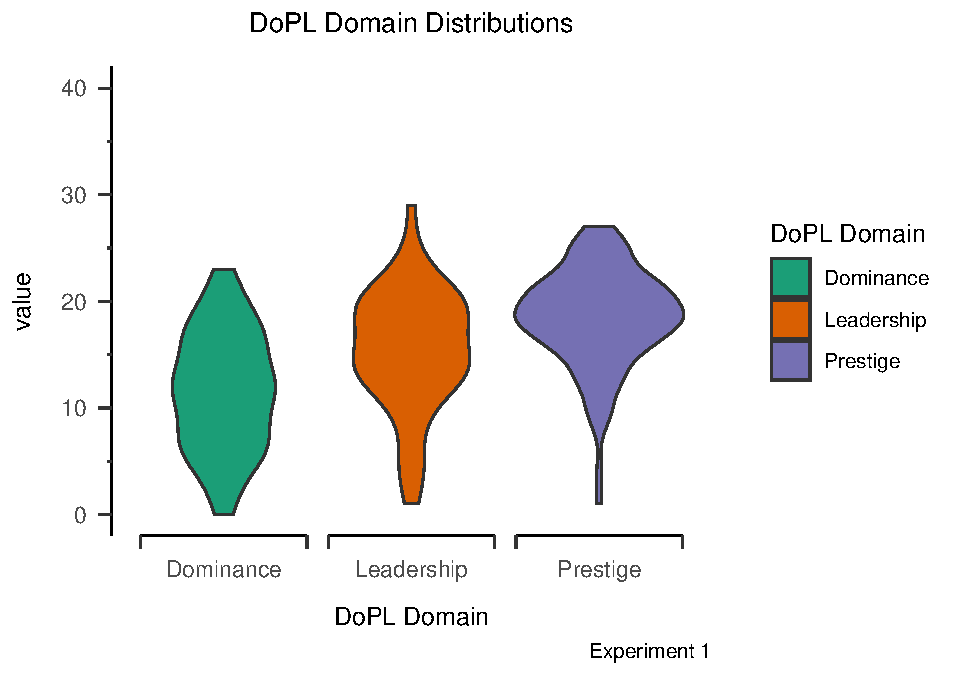
\includegraphics{Output_Files/DoPL-Experiment_files/figure-latex/Dominance, Prestige, and Leadership Distribution-1.pdf}
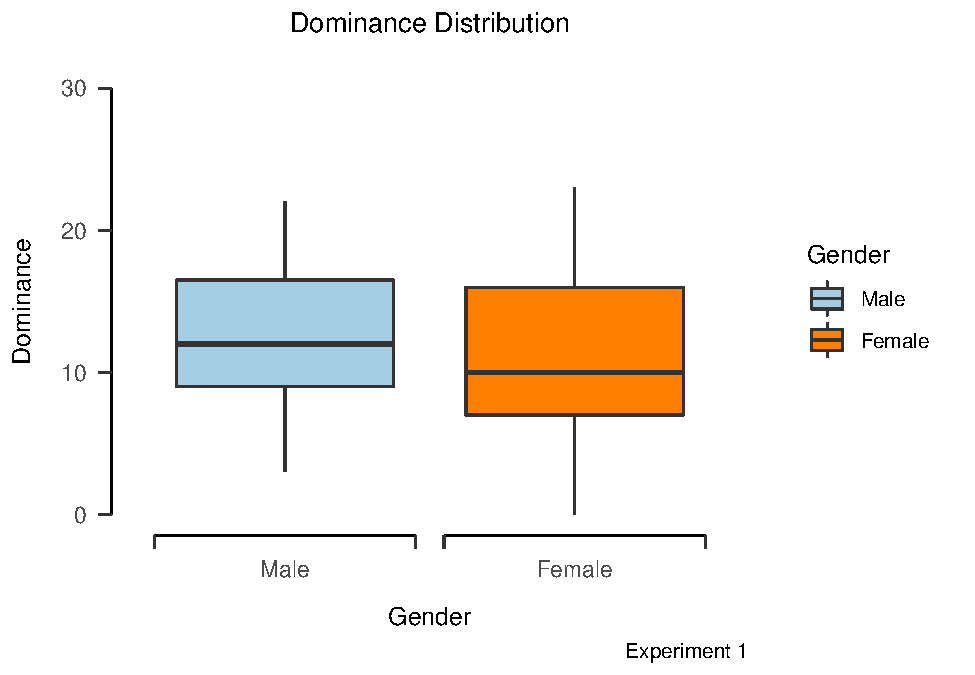
\includegraphics{Output_Files/DoPL-Experiment_files/figure-latex/Dominance-1.pdf}
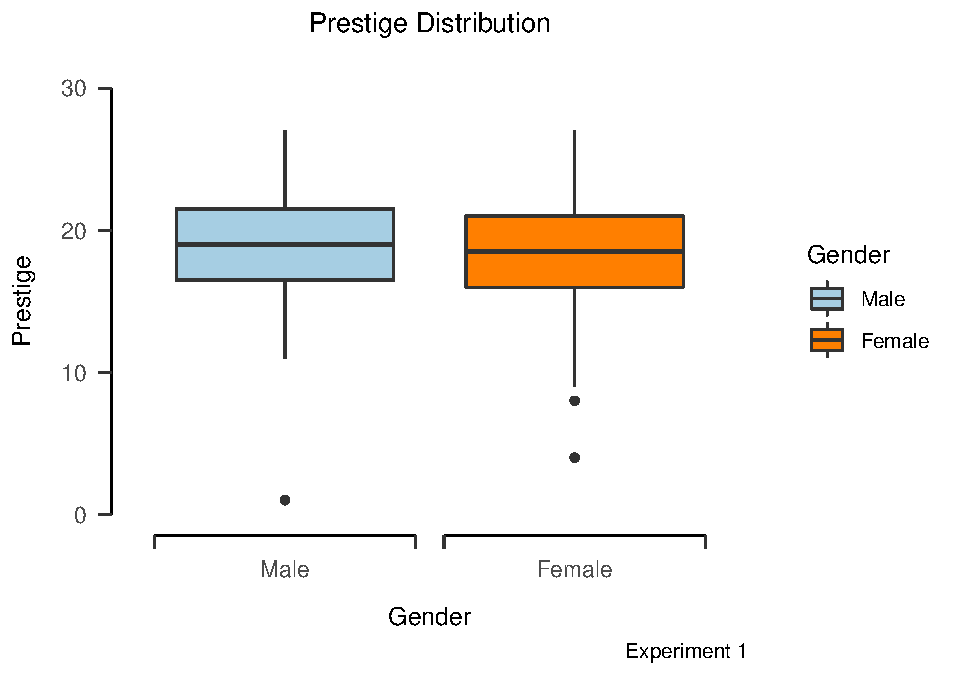
\includegraphics{Output_Files/DoPL-Experiment_files/figure-latex/Prestige-1.pdf}
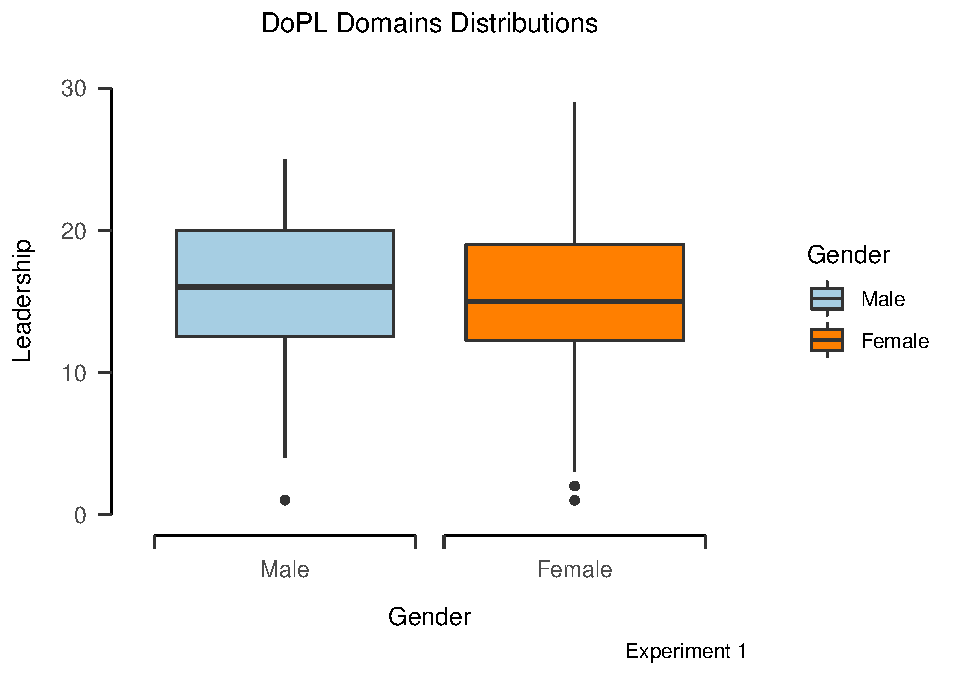
\includegraphics{Output_Files/DoPL-Experiment_files/figure-latex/Leadership-1.pdf}
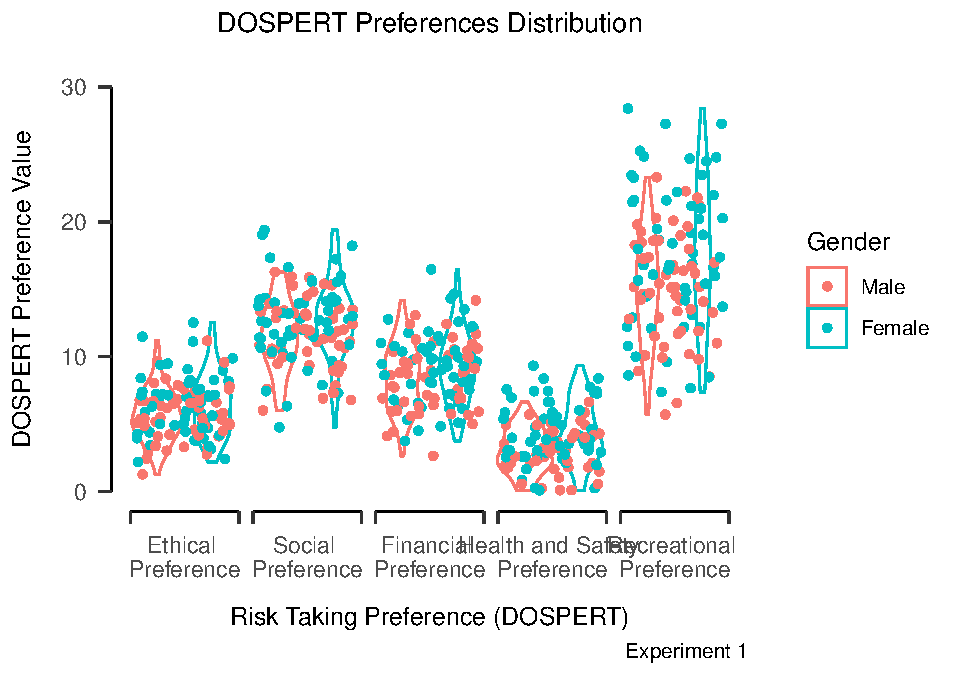
\includegraphics{Output_Files/DoPL-Experiment_files/figure-latex/DOSPERT Preferences_Gender-1.pdf}
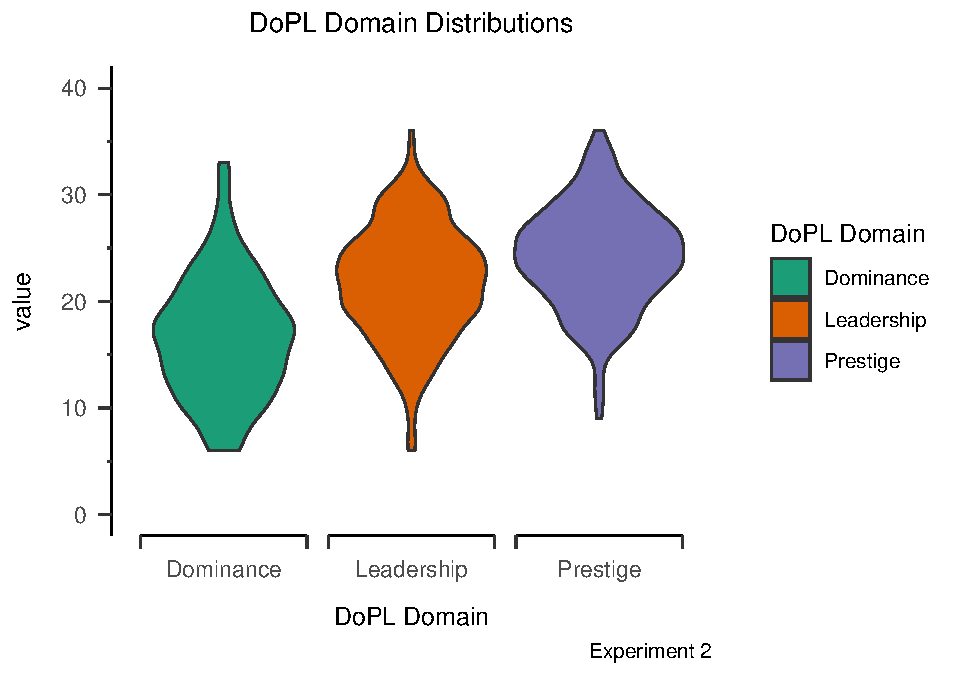
\includegraphics{Output_Files/DoPL-Experiment_files/figure-latex/DoPL Domains Experiment 2-1.pdf}
\newpage
\hypertarget{tables}{%
\subsection{Tables}\label{tables}}
\begin{table}[h]
\begin{center}
\begin{threeparttable}
\caption{\label{tab:unnamed-chunk-2}Experiment 1: Participant Demographics}
\begin{tabular}{ll}
\toprule
Characteristic & N=109\\
\midrule
Age & \\
\ \ \ Mean (SD) & 27 (9.25)\\
\ \ \ Median [Range] & 24 [18.00, 61]\\
Gender & \\
\ \ \ Female & 54 (50\%)\\
\ \ \ Male & 55 (50\%)\\
Ethnicity & \\
\ \ \ African & 8 (7.3\%)\\
\ \ \ Asian & 6 (5.5\%)\\
\ \ \ English & 10 (9.2\%)\\
\ \ \ European & 76 (70\%)\\
\ \ \ Latin American & 2 (1.8\%)\\
\ \ \ Other & 5 (4.6\%)\\
\ \ \ Scottish & 2 (1.8\%)\\
Education & \\
\ \ \ A-levels or equivalent & 32 (29\%)\\
\ \ \ Doctoral Degree & 1 (0.9\%)\\
\ \ \ GCSEs or equivalent & 8 (7.3\%)\\
\ \ \ Prefer not to respond & 1 (0.9\%)\\
\ \ \ Primary School & 4 (3.7\%)\\
\ \ \ University Postgraduate Program & 21 (19\%)\\
\ \ \ University Undergraduate Program & 42 (39\%)\\
\bottomrule
\end{tabular}
\end{threeparttable}
\end{center}
\end{table}
\begin{table}[h]
\begin{center}
\begin{threeparttable}
\caption{\label{tab:unnamed-chunk-3}Fixed Effects: DoPL * General Risk}
\begin{tabular}{lllll}
\toprule
Parameter & \multicolumn{1}{c}{Estimate} & \multicolumn{1}{c}{CI} & \multicolumn{1}{c}{CI Low} & \multicolumn{1}{c}{CI High}\\
\midrule
Intercept & 3.62 & 0.95 & 1.41 & 5.86\\
Dominance & 3 & 0.95 & 1.08 & 4.93\\
Gender & -3.02 & 0.95 & -4.95 & -1.08\\
Age & -2.86 & 0.95 & -4.78 & -0.93\\
\bottomrule
\addlinespace
\end{tabular}
\begin{tablenotes}[para]
\normalsize{\textit{Note.} Table 2 represents fixed effects, confidence interevals low and high for a basic bayesian model of Dominance, Prestige, and Leadership predicting general risk preference. Matching signs for confidence intervals is displayed in the table.}
\end{tablenotes}
\end{threeparttable}
\end{center}
\end{table}
\begin{table}[h]
\begin{center}
\begin{threeparttable}
\caption{\label{tab:m1_int_fixef_exp_1}DOSPERT and DoPL Interaction: Experiment 1}
\begin{tabular}{lllll}
\toprule
Parameter & \multicolumn{1}{c}{Estimate} & \multicolumn{1}{c}{CI} & \multicolumn{1}{c}{CI Low} & \multicolumn{1}{c}{CI High}\\
\midrule
Ethical Preference * Intercept & 3.61 & 0.95 & 2.79 & 4.37\\
Financial Preference * Intercept & 8.6 & 0.95 & 7.47 & 9.66\\
Social Preference * Intercept & 9.98 & 0.95 & 8.27 & 11.64\\
Health and Safety Preference * Intercept & 5.6 & 0.95 & 4.6 & 6.54\\
Recreational Preference * Intercept & 1.68 & 0.95 & 0.86 & 2.43\\
Ethical Preference * Dominance & 1.15 & 0.95 & 0.61 & 1.71\\
Financial Preference * Dominance & 0.87 & 0.95 & 0.13 & 1.58\\
Social Preference * Dominance & 1.81 & 0.95 & 0.64 & 2.94\\
Health and Safety Preference * Dominance & 1.09 & 0.95 & 0.41 & 1.77\\
Recreational Preference * Dominance & 1.22 & 0.95 & 0.67 & 1.76\\
Recreational Preference * Gender & -1.14 & 0.95 & -1.83 & -0.47\\
Recreational Preference * Age & 0.46 & 0.95 & 0.05 & 0.86\\
\bottomrule
\addlinespace
\end{tabular}
\begin{tablenotes}[para]
\normalsize{\textit{Note.} Fixed effect results of Dominance, Prestige, and Leadership with gender interactions predicting each of the individual Domain Specific Risk Taking (DOSPERT) domains.}
\end{tablenotes}
\end{threeparttable}
\end{center}
\end{table}
\begin{table}[h]
\begin{center}
\begin{threeparttable}
\caption{\label{tab:m5_int_fixef_exp_1}DOSPERT Benefit and Perception: Experiment 1}
\begin{tabular}{lllll}
\toprule
Parameter & \multicolumn{1}{c}{Estimate} & \multicolumn{1}{c}{CI} & \multicolumn{1}{c}{CI Low} & \multicolumn{1}{c}{CI High}\\
\midrule
Risk * Dominance & 0.65 & 0.95 & 0.36 & 0.95\\
Risk * Gender & -0.5 & 0.95 & -0.85 & -0.14\\
Risk * Dominance : Gender & -0.48 & 0.95 & -0.85 & -0.11\\
Risk Perception * Gender & 0.43 & 0.95 & 0.05 & 0.8\\
Risk Perception * Prestige & 0.31 & 0.95 & 0.01 & 0.61\\
Risk Perception * Leadership : Gender & 0.43 & 0.95 & 0.03 & 0.82\\
Risk Benefit * Dominance & 0.38 & 0.95 & 0.07 & 0.71\\
Risk Benefit * Gender & -0.6 & 0.95 & -0.98 & -0.22\\
\bottomrule
\addlinespace
\end{tabular}
\begin{tablenotes}[para]
\normalsize{\textit{Note.} Fixed effect results of Dominance, Prestige, and Leadership with gender interactions predicting the perceptions and benefits of risk.}
\end{tablenotes}
\end{threeparttable}
\end{center}
\end{table}
\begin{table}[h]
\begin{center}
\begin{threeparttable}
\caption{\label{tab:m4_perceivedRisk_Gender_exp_1}DOSPERT Benefit and Perception: Experiment 1}
\begin{tabular}{lllll}
\toprule
Parameter & \multicolumn{1}{c}{Estimate} & \multicolumn{1}{c}{CI} & \multicolumn{1}{c}{CI Low} & \multicolumn{1}{c}{CI High}\\
\midrule
Ethical Perception * Prestige & 0.39 & 0.95 & 0.12 & 0.66\\
Recreational Perception * Prestige & 0.33 & 0.95 & 0.06 & 0.6\\
Recreational Perception * Age & -0.22 & 0.95 & -0.4 & -0.04\\
Recreational Perception * Dominance : Gender & -0.4 & 0.95 & -0.77 & -0.04\\
Health and Safety Perception * Leadership : Gender & 0.44 & 0.95 & 0.07 & 0.8\\
\bottomrule
\addlinespace
\end{tabular}
\begin{tablenotes}[para]
\normalsize{\textit{Note.} Fixed effect results of Dominance, Prestige, and Leadership with gender interactions predicting the perceptions and benefits of risk.}
\end{tablenotes}
\end{threeparttable}
\end{center}
\end{table}
\begin{table}[h]
\begin{center}
\begin{threeparttable}
\caption{\label{tab:Experiment 2: Participant Demographics}Experiment 2: Participant Demographics}
\begin{tabular}{ll}
\toprule
Characteristic & N=279\\
\midrule
Age & \\
\ \ \ Mean (SD) & 30 (9.92)\\
\ \ \ Median [Range] & 26 [18.00, 78]\\
Gender & \\
\ \ \ Female & 124 (44\%)\\
\ \ \ Male & 155 (56\%)\\
Ethnicity & \\
\ \ \ African & 49 (18\%)\\
\ \ \ Asian  or  Asian Scottish  or  Asian British & 5 (1.8\%)\\
\ \ \ Mixed  or  Multi-ethnic & 7 (2.5\%)\\
\ \ \ Other ethnicity & 3 (1.1\%)\\
\ \ \ Prefer not  to respond & 1 (0.4\%)\\
\ \ \ White & 214 (77\%)\\
Education & \\
\ \ \ A-Levels  or  Equivalent & 64 (23\%)\\
\ \ \ Doctoral  Degree & 4 (1.4\%)\\
\ \ \ GCSEs  or  Equivalent & 17 (6.1\%)\\
\ \ \ Prefer not  to respond & 4 (1.4\%)\\
\ \ \ Primary School & 5 (1.8\%)\\
\ \ \ University  Post-Graduate  Program & 62 (22\%)\\
\ \ \ University  Undergraduate  Program & 123 (44\%)\\
Ethnic Origin & \\
\ \ \ African & 48 (17\%)\\
\ \ \ Asian & 7 (2.5\%)\\
\ \ \ English & 16 (5.7\%)\\
\ \ \ European & 193 (69\%)\\
\ \ \ Latin American & 6 (2.2\%)\\
\ \ \ Other & 9 (3.2\%)\\
\bottomrule
\end{tabular}
\end{threeparttable}
\end{center}
\end{table}
\begin{table}[h]
\begin{center}
\begin{threeparttable}
\caption{\label{tab:PNI Model DoPL Exp 2}General Risk * DoPL: Experiment 2}
\begin{tabular}{lllll}
\toprule
Parameter & \multicolumn{1}{c}{Estimate} & \multicolumn{1}{c}{CI} & \multicolumn{1}{c}{CI Low} & \multicolumn{1}{c}{CI High}\\
\midrule
Intercept & 0.81 & 0.95 & 0.4 & 1.22\\
Dominance & 0.51 & 0.95 & 0.17 & 0.86\\
Prestige & 0.42 & 0.95 & 0.07 & 0.78\\
Age & -0.02 & 0.95 & -0.03 & -0.01\\
\bottomrule
\addlinespace
\end{tabular}
\begin{tablenotes}[para]
\normalsize{\textit{Note.} Fixed effect results of Dominance, Prestige, and Leadership with gender interactions predicting general risk preference.}
\end{tablenotes}
\end{threeparttable}
\end{center}
\end{table}
\begin{table}[h]
\begin{center}
\begin{threeparttable}
\caption{\label{tab:Vulnerability and Grandiosity_DOSPERT}B-PNI * DOSPERT : Gender: Experiment 2}
\begin{tabular}{lllll}
\toprule
Parameter & \multicolumn{1}{c}{Estimate} & \multicolumn{1}{c}{CI} & \multicolumn{1}{c}{CI Low} & \multicolumn{1}{c}{CI High}\\
\midrule
Vulnerability * Intercept & 0.82 & 0.95 & 0.44 & 1.21\\
Vulnerability * Financial Preference & -0.27 & 0.95 & -0.47 & -0.06\\
Vulnerability * Age & -0.03 & 0.95 & -0.04 & -0.02\\
Vulnerability * Recreational Preference : Gender & -0.34 & 0.95 & -0.62 & -0.07\\
Grandiosity * Gender & 0.27 & 0.95 & 0.03 & 0.51\\
Grandiosity * Social Preference & 0.3 & 0.95 & 0.11 & 0.49\\
Grandiosity * Recreational Preference : Gender & -0.41 & 0.95 & -0.69 & -0.13\\
\bottomrule
\addlinespace
\end{tabular}
\begin{tablenotes}[para]
\normalsize{\textit{Note.} Fixed effect results of individual DOSPERT domains with gender interactions predicting vulnerable and grandiose narcissism respectivley.}
\end{tablenotes}
\end{threeparttable}
\end{center}
\end{table}
\hypertarget{refs}{}
\begin{CSLReferences}{1}{0}
\leavevmode\vadjust pre{\hypertarget{ref-anderson2012}{}}%
Anderson, C., John, O. P., \& Keltner, D. (2012). The personal sense of power. \emph{Journal of Personality}, \emph{80}(2), 313--344. \url{https://doi.org/10.1111/j.1467-6494.2011.00734.x}
\leavevmode\vadjust pre{\hypertarget{ref-aust2020}{}}%
Aust, F., \& Barth, M. (2020). \emph{Papaja: {Prepare} reproducible {APA} journal articles with {R Markdown}}.
\leavevmode\vadjust pre{\hypertarget{ref-bareket2020}{}}%
Bareket, O., \& Shnabel, N. (2020). Domination and objectification: Men's motivation for dominance over women affects their tendency to sexually objectify women. \emph{Psychology of Women Quarterly}, \emph{44}(1), 28--49. \url{https://doi.org/10.1177/0361684319871913}
\leavevmode\vadjust pre{\hypertarget{ref-bernstein2020}{}}%
Bernstein, R. (2020). The paradox of rodrigo duterte. \emph{The Atlantic}.
\leavevmode\vadjust pre{\hypertarget{ref-bierstedt1950}{}}%
Bierstedt, R. (1950). An analysis of social power. \emph{American Sociological Review}, \emph{15}(6), 730--738. \url{https://doi.org/10.2307/2086605}
\leavevmode\vadjust pre{\hypertarget{ref-breakwell2007}{}}%
Breakwell, G. M. (2007). The psychology of risk. In \emph{Cambridge Core}. /core/books/psychology-of-risk/3AA5E35577684DF437A1F3084CD2FA8B. \url{https://doi.org/10.1017/CBO9780511819315}
\leavevmode\vadjust pre{\hypertarget{ref-burkner2017}{}}%
Bürkner, P.-C. (2017). Brms: An {R} package for bayesian multilevel models using stan. \emph{Journal of Statistical Software}, \emph{80}(1), 1--28. \url{https://doi.org/10.18637/jss.v080.i01}
\leavevmode\vadjust pre{\hypertarget{ref-burkner2018}{}}%
Bürkner, P.-C. (2018). Advanced bayesian multilevel modeling with the {R} package brms. \emph{The R Journal}, \emph{10}(1), 395--411. \url{https://doi.org/10.32614/RJ-2018-017}
\leavevmode\vadjust pre{\hypertarget{ref-chen2021}{}}%
Chen, Z., \& John, R. S. (2021). Decision heuristics and descriptive choice models for sequential high-stakes risky choices in the deal or no deal game. \emph{Decision}, \emph{8}(3), 155--179. \url{https://doi.org/10.1037/dec0000153}
\leavevmode\vadjust pre{\hypertarget{ref-desiderato1995}{}}%
Desiderato, L. L., \& Crawford, H. J. (1995). Risky sexual behavior in college students: Relationships between number of sexual partners, disclosure of previous risky behavior, and alcohol use. \emph{Journal of Youth and Adolescence}, \emph{24}(1), 55--68. \url{https://doi.org/10.1007/BF01537560}
\leavevmode\vadjust pre{\hypertarget{ref-gabry2021}{}}%
Gabry, J., \& Cesnovar, R. (2021). \emph{Cmdstanr: {R} interface to '{CmdStan}'}.
\leavevmode\vadjust pre{\hypertarget{ref-2018}{}}%
Glamorizing dictators. (2018). In \emph{Towson University Journal of International Affairs}.
\leavevmode\vadjust pre{\hypertarget{ref-johnson2012}{}}%
Johnson, M. W., \& Bruner, N. R. (2012). The sexual discounting task: {HIV} risk behavior and the discounting of delayed sexual rewards in cocaine dependence. \emph{Drug and Alcohol Dependence}, \emph{123}(1-3), 15--21. \url{https://doi.org/10.1016/j.drugalcdep.2011.09.032}
\leavevmode\vadjust pre{\hypertarget{ref-johnson2015a}{}}%
Johnson, P. S., Herrmann, E. S., \& Johnson, M. W. (2015). Opportunity costs of reward delays and the discounting of hypothetical money and cigarettes: {OPPORTUNITY COSTS AND DISCOUNTING}. \emph{Journal of the Experimental Analysis of Behavior}, \emph{103}(1), 87--107. \url{https://doi.org/10.1002/jeab.110}
\leavevmode\vadjust pre{\hypertarget{ref-king2009}{}}%
King, A. J., Johnson, D. D. P., \& Van Vugt, M. (2009). The origins and evolution of leadership. \emph{Current Biology}, \emph{19}(19), R911--R916. \url{https://doi.org/10.1016/j.cub.2009.07.027}
\leavevmode\vadjust pre{\hypertarget{ref-kirby2021}{}}%
Kirby, M. (2021). North korea on the brink of the biden administration: Human rights, peace, and security. \emph{Indiana International \& Comparative Law Review}, \emph{31}(2), 309--327.
\leavevmode\vadjust pre{\hypertarget{ref-kuhberger2009}{}}%
Kühberger, A., \& Tanner, C. (2009). Risky choice framing: Task versions and a comparison of prospect theory and fuzzy-trace theory. \emph{Journal of Behavioral Decision Making}, \emph{23}(3), 314--329. \url{https://doi.org/dtqksm}
\leavevmode\vadjust pre{\hypertarget{ref-makowski2019}{}}%
Makowski, D., Ben-Shachar, M., \& Ludecke, D. (2019). {bayestestR}: {Describing Effects} and their {Uncertainty}, {Existence} and {Significance} within the {Bayesian Framework}. \emph{Journal of Open Source Software}, \emph{4}(40). \url{https://doi.org/10.21105/joss.01541}
\leavevmode\vadjust pre{\hypertarget{ref-maner2016}{}}%
Maner, J. K., \& Case, C. R. (2016). Dominance and prestige. In \emph{Advances in {Experimental Social Psychology}} (Vol. 54, pp. 129--180). {Elsevier}. \url{https://doi.org/10.1016/bs.aesp.2016.02.001}
\leavevmode\vadjust pre{\hypertarget{ref-petersen2018}{}}%
Petersen, R. M., Dubuc, C., \& Higham, J. P. (2018). Facial displays of dominance in non-human primates. In C. Senior (Ed.), \emph{The {Facial Displays} of {Leaders}} (pp. 123--143). {Springer International Publishing}. \url{https://doi.org/10.1007/978-3-319-94535-4_6}
\leavevmode\vadjust pre{\hypertarget{ref-pincus2009}{}}%
Pincus, A. L., Ansell, E. B., Pimentel, C. A., Cain, N. M., Wright, A. G. C., \& Levy, K. N. (2009). Initial construction and validation of the {Pathological Narcissism Inventory}. \emph{Psychological Assessment}, \emph{21}(3), 365--379. \url{https://doi.org/10.1037/a0016530}
\leavevmode\vadjust pre{\hypertarget{ref-prolificacademic2018}{}}%
Prolific Academic. (2018). \emph{How do participants find out about my study?} https://researcher-help.prolific.co/hc/en-gb/articles/360009221253-How-do-participants-find-out-about-my-study-.
\leavevmode\vadjust pre{\hypertarget{ref-rcoreteam2021}{}}%
R Core Team. (2021). \emph{R: {A} language and environment for statistical computing}. R Foundation for Statistical Computing.
\leavevmode\vadjust pre{\hypertarget{ref-rosenthal2012}{}}%
Rosenthal, L., Levy, S. R., \& Earnshaw, V. A. (2012). Social dominance orientation relates to believing men should dominate sexually, sexual self-efficacy, and taking free female condoms among undergraduate women and men. \emph{Sex Roles}, \emph{67}(11-12), 659--669. \url{https://doi.org/10.1007/s11199-012-0207-6}
\leavevmode\vadjust pre{\hypertarget{ref-schoenleber2015}{}}%
Schoenleber, M., Roche, M. J., Wetzel, E., Pincus, A. L., \& Roberts, B. W. (2015). Development of a brief version of the pathological narcissism inventory. \emph{Psychological Assessment}, \emph{27}(4), 1520--1526. \url{https://doi.org/10.1037/pas0000158}
\leavevmode\vadjust pre{\hypertarget{ref-schonbrodt2012}{}}%
Schönbrodt, F. D., \& Gerstenberg, F. X. R. (2012). An {IRT} analysis of motive questionnaires: {The Unified Motive Scales}. \emph{Journal of Research in Personality}, \emph{46}(6), 725--742. \url{https://doi.org/10.1016/j.jrp.2012.08.010}
\leavevmode\vadjust pre{\hypertarget{ref-shearer2005}{}}%
Shearer, C. L., Hosterman, S. J., Gillen, M. M., \& Lefkowitz, E. S. (2005). Are traditional gender role attitudes associated with risky sexual behavior and condom-related beliefs? \emph{Sex Roles}, \emph{52}(5-6), 311--324. \url{https://doi.org/10.1007/s11199-005-2675-4}
\leavevmode\vadjust pre{\hypertarget{ref-sidanius2000}{}}%
Sidanius, J., Levin, S., Liu, J., \& Pratto, F. (2000). Social dominance orientation, anti-egalitarianism and the political psychology of gender: An extension and cross-cultural replication. \emph{European Journal of Social Psychology}, \emph{30}(1), 41--67. \url{https://doi.org/10.1002/(SICI)1099-0992(200001/02)30:1\%3C41::AID-EJSP976\%3E3.0.CO;2-O}
\leavevmode\vadjust pre{\hypertarget{ref-standevelopmentteam2020}{}}%
Stan Development Team. (2020). \emph{{RStan}: The {R} interface to stan}.
\leavevmode\vadjust pre{\hypertarget{ref-suessenbach2019}{}}%
Suessenbach, F., Loughnan, S., Schönbrodt, F. D., \& Moore, A. B. (2019). The dominance, prestige, and leadership account of social power motives. \emph{European Journal of Personality}, \emph{33}(1), 7--33. \url{https://doi.org/10.1002/per.2184}
\leavevmode\vadjust pre{\hypertarget{ref-vanvugt2006}{}}%
Van Vugt, M. (2006). Evolutionary origins of leadership and followership. \emph{Personality and Social Psychology Review}, \emph{10}(4), 354--371. \url{https://doi.org/10.1207/s15327957pspr1004_5}
\leavevmode\vadjust pre{\hypertarget{ref-vugt2014}{}}%
Vugt, M. van, \& Ronay, R. (2014). The evolutionary psychology of leadership: Theory, review, and roadmap. \emph{Organizational Psychology Review}, \emph{4}(1), 74--95. \url{https://doi.org/10.1177/2041386613493635}
\leavevmode\vadjust pre{\hypertarget{ref-weber2002}{}}%
Weber, E. U., Blais, A.-R., \& Betz, N. E. (2002). A domain-specific risk-attitude scale: Measuring risk perceptions and risk behaviors. \emph{Journal of Behavioral Decision Making}, \emph{15}(4), 263--290. \url{https://doi.org/10.1002/bdm.414}
\leavevmode\vadjust pre{\hypertarget{ref-winter1993}{}}%
Winter, D. G. (1993). Power, affiliation, and war: Three tests of a motivational model. \emph{Journal of Personality and Social Psychology}, \emph{65}(3), 532--545. \url{https://doi.org/10.1037/0022-3514.65.3.532}
\leavevmode\vadjust pre{\hypertarget{ref-witkower2020}{}}%
Witkower, Z., Tracy, J. L., Cheng, J. T., \& Henrich, J. (2020). Two signals of social rank: Prestige and dominance are associated with distinct nonverbal displays. \emph{Journal of Personality and Social Psychology}, \emph{118}(1), 89--120. \url{https://doi.org/10.1037/pspi0000181}
\end{CSLReferences}
\end{document}
